% !TeX root = ../main.tex

\chapter{相关技术概述}
本章简单阐述系统开发中使用到的关键技术,并简要分析了其与CI/CD系统相关性和适用性,
包括CI/CD流水线概念与实践、Docker容器化技术、容器集群调度引擎Kubernetes、 GitLab Runner和消息队列RocketMQ。

\section{CI/CD流水线}
软件开发领域的“流水线”概念来源于工业上的产品流水线。
工业流水线指的是每个生产单位专注于处理某个片段的工作,以提高工作效率和产量。
CI/CD流水线与之类似,将软件开发中的各个环节拆分,产生一条标准化的研发流程,在流水线的运行中产生不断更迭的软件版本。
在一个软件产品的迭代过程中,会有一系列的研发阶段,从需求收集开始,经过编译、测试、部署等阶段,最终会产生软件的一个版本,
而在当今以敏捷开发为主流的模式下,这一套流程会被不断的重复,从而成为一套自动化的流水线。图~\ref{fig:典型流水线示意图} 是一条典型的CI/CD流水线包含的内容。

\begin{figure}[h]
    \centering
    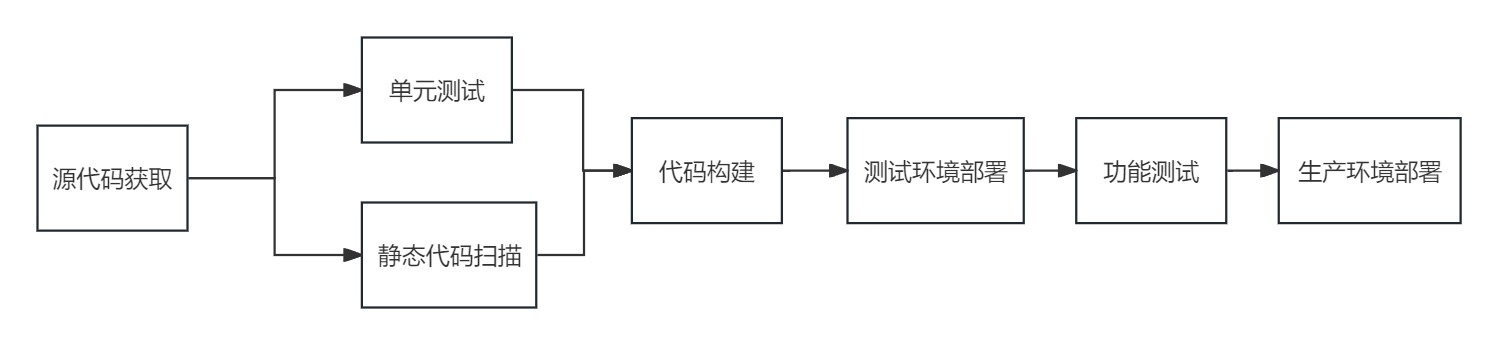
\includegraphics[width=1\textwidth]{典型流水线示意图.jpg}
    \caption{典型流水线示意图}
    \label{fig:典型流水线示意图}
  \end{figure}

CI/CD流水线使得软件的开发、测试和交付变得更加高效、可靠和可控\cite{mohammad2016continuous}。
同时,这种自动化的流程有助于加速软件交付周期,减少人工操作带来的错误,并提高整体团队的协作效率。

\section{Docker容器化技术}
容器化技术是一种轻量级的虚拟化方法,通过将应用程序及其依赖项打包到一个独立的、可移植的容器中,实现了在不同环境中一致性的部署和运行。
基于Docker的容器化技术在这一领域取得了显著的成功。

Docker 是一个由 Golang 语言开发的,开源的容器化平台,它采用了操作系统层面的虚拟化技术,允许开发人员将应用程序及其所有依赖项打包为一个称为容器的标准单元\cite{第二章Docker}。
这个容器包括应用程序的代码、运行时、系统工具、系统库和设置,确保在不同的环境中能够以一致的方式运行。

Docker容器与传统的虚拟机技术(VM)有一定相似之处,但又拥有着一系列优势。首先,Docker 容器在资源利用率方面表现出色\cite{张忠琳2014基于}。与传统虚拟机相比,它们不需要为每个虚拟机加载一个完整的操作系统,而是与宿主机共享核心,这大大减少了硬盘使用、内存占用和启动时间。
此外,Docker 容器提供了更高的效率和更快的部署速度,使得在几秒钟内就可以创建和启动容器,而虚拟机可能需要几分钟\cite{JSJY201704001}。
Docker 容器还促进了环境一致性,确保应用程序在开发、测试和生产环境中运行时的一致性和可预测性。
最后,Docker 的生态系统和工具链提供了广泛的支持\cite{DGJB201806026},包括容器编排、管理和安全,这些都是在现代云原生应用开发中不可或缺的部分。
Docker容器与传统虚拟机的对比如表~\ref{tab:Docker容器与传统虚拟机对比}所示。

\begin{table}[h]
  \centering
  \caption{Docker容器与传统虚拟机对比}
  \label{tab:Docker容器与传统虚拟机对比}
  \begin{tabular}{lcc}
    \toprule
      特性           & Docker 容器            & 传统虚拟机               \\
    \midrule
      启动时间       & 秒级                   & 分钟级                   \\
      硬盘使用       & 一般为MB               & 一般为GB                  \\
      性能           & 接近原生               & 较低   \\
      资源占用       & 低                     & 高                       \\
      系统支持数量   & 单机支持上千个容器       & 一般为几十个              \\
      部署速度       & 快                     & 慢                        \\
      环境一致性     & 高                     & 中等,受到底层VM配置的影响  \\
    \bottomrule
  \end{tabular}
  \end{table}

Docker中有两个基本概念:镜像和容器,这是CI/CD系统实现容器化的基础\cite{boettiger2015introduction}。

Docker 镜像是一个轻量级、可执行的软件包,包含了应用程序的代码、运行时、系统工具、系统库和设置。
镜像的构建规则通过 Dockerfile 文件定义,形成一个静态的快照,具有版本控制和分层结构,确保了构建的可重复性和高效性。
这些镜像可以被推送到 Docker 镜像仓库,以供后续的CI/CD环节使用。

Docker 容器是基于 Docker 镜像运行的实例,拥有独立的命名空间、进程空间、文件系统、网络配置和用户ID空间,提供了一个隔离的执行环境。
每个容器都是独立的运行单元,可以快速启动、停止和删除。
容器解决了环境一致性的问题,确保应用程序在不同的阶段和环境中能够以相同的方式运行。
容器的快速部署和回滚特性加速了CI/CD流程,使得团队能够更灵活、高效地进行应用程序的开发、测试和部署。

以下是 Docker 的关键特点和为何它适用于CI/CD系统的原因:

\paragraph{轻量级}Docker容器比虚拟机更轻量,容器的启动与销毁都是秒级,同时占用更少的资源。

\paragraph{一致性}Docker提供一致的运行环境,当Docker镜像被打包好以后,所有根据该镜像启动的容器拥有完全一致、标准化的环境。

\paragraph{可移植性}Docker容器可以在任何支持 Docker 引擎的环境中运行,无论是开发者的本地机器、测试服务器还是生产环境。这种可移植性确保了应用程序在不同阶段和环境中的一致性,简化了部署流程。

\paragraph{隔离性}Docker提供了一定程度的隔离,每个容器都运行在独立的用户空间中,不受其他容器或宿主系统的影响。这种隔离性确保了不同的流水线作业可以并行运行,同时避免了冲突和资源争用\cite{JSJC201708006}。

\paragraph{快速构建和部署}Docker的快速构建能力使得在CI/CD过程中能够更迅速地生成新的镜像,同时容器的快速启动和停止加速了部署过程。这对于频繁进行集成和部署的 CI/CD 系统至关重要。

基于以上特性,Docker几乎成为当今Devops以及CI/CD实践中不可或缺的完美解决方案\cite{第二章Devops}。

\section{容器集群调度引擎Kubernetes}
在现代软件开发领域,Kubernetes(K8s)已经成为最受欢迎的容器集群调度引擎之一,特别是在CI/CD流程的高效实现中展示了其无与伦比的优势\cite{XTYY202012038}\cite{mahboob2021kubernetes}。

Kubernetes不仅促进了DevOps文化的快速发展,还为敏捷开发提供了坚实的技术支持,极大地提高了研发团队交付高质量软件产品的能力\cite{carrion2022kubernetes}。

Kubernetes与Docker之间的关系构成了容器化技术生态系统的核心\cite{XDDS202202023}。
Docker作为容器技术的领导者,为应用提供了轻量级和可移植的封装环境。
Kubernetes则为这些容器提供了自动化的部署、扩展和管理平台。
通过将Docker容器部署到Kubernetes集群中,开发团队能够以前所未有的灵活性和自动化水平管理服务的生命周期,包括部署、扩展和更新。这种结合最大化地利用了Docker容器的隔离性和资源轻量化的优点,并通过Kubernetes的管理能力实现了更高级的自动化操作和系统灵活性。

Kubernetes的设计理念是提供一个分布式系统友好的环境,支持多种容器工具和跨云及本地部署,这使得它成为企业实现云原生应用的关键工具。其架构中包含多个关键组件,例如控制平面、节点、Pod以及服务,这些组件共同工作以确保应用的高可用性和可扩展性,并提供了负载均衡、自我修复、服务发现和配置管理等关键功能。

在CI/CD系统中,Kubernetes提供的自动化和灵活性特性尤其突出\cite{janani2022analysis}。它能够自动化CI/CD流程的各个阶段,支持声明式配置和自动化部署,使得应用的更新和回滚过程无需人工干预。此外,Kubernetes的服务发现和负载均衡功能使得服务间的通信变得更加高效,为基于微服务架构的应用提供了坚实的基础。

Kubernetes在横向扩展和故障转移方面的能力非常出色\cite{JSSG201909023}。它可以根据应用负载自动增加或减少容器实例的数量,同时监控容器健康状态并在必要时自动替换故障容器,确保了系统的高可用性。这种弹性不仅优化了资源利用率,还支持了应用性能的维护。

Kubernetes的生态系统是其另一个显著特点,随着行业内的广泛采用,出现了大量围绕Kubernetes开发的工具和扩展,如Helm、Prometheus、Istio和Knative。这些工具和扩展进一步增强了Kubernetes的功能,支持复杂的微服务架构和无服务器计算。

综上所述,Kubernetes通过其与Docker的深度整合、对DevOps实践的支持、在自动化、扩展性和可靠性方面的优势,成为构建现代软件开发管道的理想选择。其在促进软件快速开发和迭代、提高系统稳定性和可靠性方面的能力,为企业创造了巨大的业务价值,使其在实现敏捷开发和持续集成/持续部署(CI/CD)过程中扮演了不可或缺的角色。


\section{GitLab Runner}
GitLab Runner是一个开源项目,是Gitlab中CI/CD Pipeline服务中的一个核心组件,用于运行用户定义的的CI/CD作业并发送结果回GitLab\cite{eguzo2023automating}。
用户在使用GitLab代码管理服务时,可以仓库中添加以".gitlab-ci.yaml"为后缀的文件以定义流水线的配置与结构,同时完成GitLab Runner的相关设置,即可在GitLab中使用流水线服务。

GitLab Runner的设计和实现体现了敏捷开发和研发效能的提升。它能够并行执行多个作业,并且可以根据项目的需求动态地扩展和缩减计算资源,极大地提高了资源的利用效率和作业的执行速度。此外,GitLab Runner提供了丰富的执行器选项,包括Shell、SSH、Docker等,用户可以根据自己的需求选择最合适的执行器。例如,在容器化的CI/CD流水线中,Docker执行器允许每个作业在隔离的容器环境中运行,这不仅提高了作业的安全性,也保证了环境之间的一致性。

GitLab Runner的灵活性和可扩展性使其不仅在GitLab CI的场景下发挥作用,还可以被复用到其他系统中。
借助GitLab Runner,开发团队可以构建一个高度定制化的CI/CD环境,将自动化测试、代码部署等步骤无缝集成。由于其开放性和模块化设计,GitLab Runner可以与市场上的大多数主流技术栈兼容,这意味着企业可以在不重建整个CI/CD系统的情况下,将GitLab Runner集成进现有的工作流程中。

进一步地,GitLab Runner对于提高研发效能可以起到重要作用。
它支持缓存依赖项和工件,可以显著减少构建时间,并且能够自动化执行复杂的部署策略,从而加快从开发到部署的整个过程。
同时,GitLab Runner提供了详细的日志和历史记录,使得问题定位和性能监控变得更加高效\cite{vassallo2020configuration}。

在容器化的CI/CD流水线中,GitLab Runner与Docker、Kubernetes等技术的结合尤为紧密。它不仅能够在Docker容器中运行作业,还能够在Kubernetes集群中进行作业调度,这大大增强了其在容器化环境下的适用性和效率。此外,通过与消息队列系统如RocketMQ的集成,GitLab Runner可以更好地管理作业队列,优化资源分配,进一步提高流水线的性能和稳定性。

总而言之,GitLab Runner不仅是实现持续集成、持续交付的关键组件,它的高度可配置性和强大功能也使其成为了连接开发、测试和部署各环节的重要纽带。通过充分利用GitLab Runner,企业不仅能够构建高效、可靠的CI/CD流水线,还能够提升整个软件开发生命周期的质量和效率。因此,在自研的CI/CD流水线系统中深入整合和优化GitLab Runner,将为实现更敏捷、更高效的研发流程提供坚实的基础。


\section{消息队列RocketMQ}
RocketMQ是由阿里巴巴最初开发,并于2016年捐赠给Apache软件基金会的开源分布式消息队列中间件。
所谓消息队列,是一种遵循先进先出规则的高级数据结构,生产者将消息推送到消息队列中,消费者则按照次序从消息队列中获取消息,RocketMQ就是消息队列的一种。
相比与其他消息队列中间件,RocketMQ在处理重复消费、延迟消息、顺序性消息和延迟消息上有着独特的解决方案,是现今最广泛使用的消息中间件之一\cite{分布式消息系统研究综述}。

RocketMQ具备高可靠、高性能、高可用等特点。它支持丰富的消息通信模式,包括顺序消息、延时消息和批量消息等,满足不同场景下的消息处理需求\cite{RJSJ201811013}。
在容器化CI/CD流水线中,这些特性使得RocketMQ成为连接各个组件、传递任务指令和状态信息的理想选择\cite{1023416528.nh}。
通过利用RocketMQ,开发团队可以确保代码提交后的各项任务,如构建、测试和部署能够准确无误且高效地执行。

RocketMQ的高扩展性和高可用性对于构建现代化的CI/CD系统尤为重要。它能够支持上万亿级别的消息堆积,为系统提供强大的数据处理能力。此外,RocketMQ的分布式特性意味着它能够在不同的服务器节点间自动分配消息,实现负载均衡,并且在节点发生故障时,能够快速进行故障转移,保证CI/CD流水线的高可用性和稳定性。

在敏捷开发的环境下,开发、测试和部署过程频繁且迭代速度快。RocketMQ的低延迟和高吞吐量特性可以确保消息在系统内部快速流转,不会成为提升研发效能的瓶颈。
此外,RocketMQ支持跨语言的客户端,这意味着不同的服务可以使用最适合自己的技术栈,同时能够通过RocketMQ高效地进行通信。

对于任务调度而言,RocketMQ提供了稳定可靠的消息保障机制。无论是在Docker容器内还是在Kubernetes集群中,RocketMQ都能保证消息的正确送达和顺序处理。
在CI/CD流水线中,各个微服务、构建任务和测试用例经常需要根据特定的顺序和条件来触发和执行,RocketMQ的消息顺序控制和消息事务功能确保了整个流程的有序性和一致性\cite{1018841702.nh}。

总结来说,RocketMQ在容器化CI/CD流水线调度系统中发挥着核心作用。它不仅提供了高效、可靠的消息服务,还支持系统的高可用性和可扩展性,是连接持续集成和持续交付各个环节的重要纽带。通过合理利用RocketMQ,可以大大提高研发团队的工作效率,加快产品从开发到上线的整个流程,同时保证系统的稳定性和可维护性。

\section{本章小结}

本章节对CI/CD流水线、Docker容器化技术、容器集群调度引擎Kubernetes、GitLab Runner以及消息队列RocketMQ等相关技术进行了详细的概述。

首先,CI/CD流水线的概念与实践为软件开发提供了一条高效、可靠、可控的自动化路径。
Docker容器化技术则在环境一致性、资源利用率、部署速度等方面带来了显著的优势。
它通过轻量级的虚拟化手段,确保了应用在开发、测试、生产等不同环境下的一致性运行,同时提升了资源的利用效率和应用的部署速度。
Kubernetes作为容器集群的调度引擎,不仅优化了容器的部署和管理,还通过其横向扩展和故障转移等能力,可以为系统提供了高可用性和高稳定性。
GitLab Runner作为GitLab CI/CD的执行器,提供了灵活的作业执行环境,支持并行执行作业、动态扩展计算资源等特性,可以为CI/CD流水线作业提供运行支持。
最后,RocketMQ作为高性能、高可靠的消息队列中间件,在容器化CI/CD流水线调度系统中扮演着消息传递的核心角色,同时完成异步和流量削峰。
以上技术各自在CI/CD系统中扮演着不可或缺的角色,并且相互协作,共同推动CI/CD流水线系统的自动化、标准化以及高效化。